\chapter{Конфигурација софтвера}

Како би могао да ефикасно проналази и отклања грешке у софтверу који развија, програмер мора имати приступ подршци за екстерно дебаговање на нивоу апстрактнијем од манипулисања линијама \textit{\acrshort{JTAG}} интерфејса. Како би ово било могуће, пре свега је потребно повезати  \textit{\acrshort{JTAG}} интерфејс циљног уређаја са десктоп рачунаром. За то се користе \textit{\acrshort{JTAG}} адаптери који повезаном рачунару омогућавају манипулацију линијама \textit{\acrshort{JTAG}} интерфејса или директан упис у \textbf{\acrshort{IR}} или \textbf{\acrshort{DR}} \textit{\acrshort{TAP}}-a (у зависности од количине логике унутар самог адаптера). У овом раду је коришћен \textit{J-Link} који у зависности од коришћеног софтвера може радити на било ком од претходно описаних нивоа апстракције.

Како би се постигао жељени ниво апстракције, потребно је додати још један слој који разуме спецификацију подршке за екстерно дебаговање повезаног чипа (у овом случају, то је \cite{debug_spec}). У овом раду су упоређена два таква софтвера: Власнички софтвер који долази уз \textit{J-Link} адаптер и \textit{Open\acrshort{OCD}} који представља решење отвореног кода. Независно од тога који се софтвер користи, потребна је одређена конфигурација како би софтвер могао правилно да комуницира са циљним уређајем. Конфигурација \textit{J-Link} софтвера се може обавити кроз аргументе командне линије или интерактивно. 

\begin{lstlisting}[language=none,caption=Интерактивна конфигурација \textit{J-Link} софтвера неопходна за повезивање на имплементирано језгро]
Type "connect" to establish a target connection, '?' for help
J-Link>connect
Please specify device / core. <Default>: RISC-V
Type '?' for selection dialog
Device>RISC-V
Please specify target interface:
J) JTAG (Default)
S) SWD
T) cJTAG
TIF>JTAG
Device position in JTAG chain (IRPre,DRPre) <Default>: -1,-1 => Auto-detect
JTAGConf>-1,-1
Specify target interface speed [kHz]. <Default>: 4000 kHz
Speed>1000
Device "RISC-V" selected.
\end{lstlisting}

Иста конфигурација се може постићи и следећим аргументима командне линије:\\ \lstinline[language=none,columns=fixed]{JLink.exe -device RISC-V -if JTAG -jtagconf -1,-1 -speed 1000 -autoconnect 1}.

Конфигурација \textit{Open\acrshort{OCD}}-а се врши кроз конфигурационе фајлове који се прослеђују као аргументи командне линије. Често се конфигурација дели на два фајла: конфигурација самог адаптера и конфигурација циљног уређаја. \textit{Open\acrshort{OCD}} 
долази са великим бројем конфигурационих фајлова за већину подржаних адаптера и велики број развојних плоча. У овом случају \textit{Open\acrshort{OCD}} пружа готов конфигурациони фајл за \textit{J-Link}, док је неопходно написати конфигурацију циљног уређаја.\newpage

\begin{lstlisting}[language=none,caption=Конфигурациони фајл циљног уређаја за \textit{Open\acrshort{OCD}} (\textbf{board\textbackslash{}custom\_riscv.cfg})]
	adapter speed 1000
	transport select jtag
	
	set _CHIPNAME riscv
	jtag newtap $_CHIPNAME cpu -irlen 5 -expected-id 0x00537291
	
	set _TARGETNAME $_CHIPNAME.cpu
	target create $_TARGETNAME.0 riscv -chain-position $_TARGETNAME
	$_TARGETNAME.0 configure -work-area-phys 0x00000000 -work-area-size 0x10000
	
	init
	
	halt
\end{lstlisting}

Како би се \textit{Open\acrshort{OCD}} правилно покренуо, потребно је навести следеће аргументе:\\ \lstinline[language=none,columns=fixed]{openocd -f "interface\jlink.cfg" -f"board\custom_riscv.cfg"}.

Као што се може видети, ове две конфигурације садрже већински исте информације: архитектуру процесора, комуникациони интерфејс и његову брзину. Конфигурациони фајл за \textit{Open\acrshort{OCD}} такође мора да садржи ширину \textbf{\acrshort{IR}} регистра и индекс \textit{\acrshort{TAP}}-a у ланцу, док \textit{J-Link} аутоматски детектује ове податке.
Очекивани идентификатор \textit{\acrshort{TAP}}-a, базна адреса и величина меморије су опциони.

Иако ови софтвери значајно подижу ниво апстракције, они немају концепт симбола јер нису свесни кода који се заправо извршава на циљном уређају. За то је потребан софтвер који, поред комуникације са циљним уређајем, разуме \textit{\acrfull{ELF}} и \textit{\acrshort{DWARF}}\footnote{За више информација о \textit{\acrshort{DWARF}}-у видети \cite{csned}.} информације за дебаговање унутар њега. Један од таквих алата је \textit{\acrshort{GDB}} који се повезује са инстанцом \textit{gdbserver}-a коју покреће \textit{Open\acrshort{OCD}} или \textit{J-Link} софтвер. Како \textit{\acrshort{GDB}} пружа само текстуални кориснички интерфејс, он се може повезати са интегрисаним развојним окружењем као што је \textit{Eclipse Embedded CDT} како би се омогућило дебаговање у комфору графичког корисничког интерфејса.

\begin{figure}[h!]
	\centering
	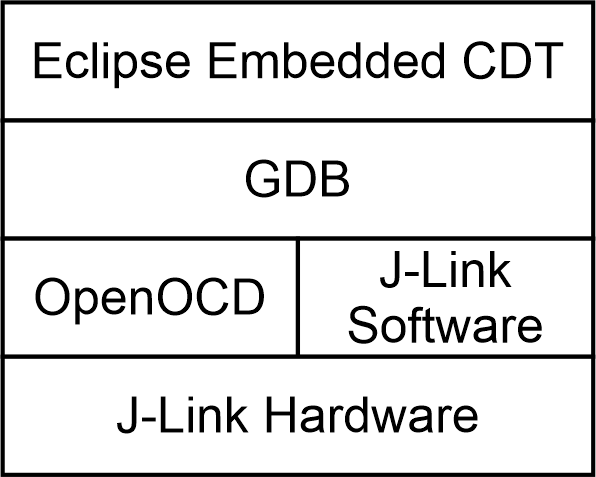
\includegraphics[width=0.35\textwidth]{stack}
	\caption{Коначни стек алата}
	\label{fig:stack}
\end{figure}

Како \textit{Eclipse Embedded CDT} има уграђену подршку за ове алате, потребно је само конфигурисати неколико параметара по упутству које се налази на званичном сајту \cite{embcdt}.
Конкретне конфигурације за \textit{Open\acrshort{OCD}} и \textit{J-Link} софтвер су приказане испод и већински садрже исте информације као конфигурације приказане раније, само у другом формату. У прилогу \ref{sec.eclipse} је приказан пример дебаговања коришћењем \textit{Eclipse Embedded CDT} интегрисаног развојног окружења.

\begin{figure}
	\centering
	\begin{minipage}{.5\textwidth}
		\centering
		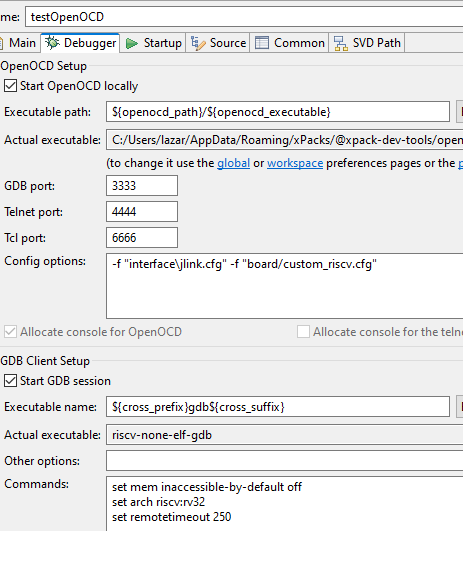
\includegraphics[width=.97\textwidth]{ocd}
		\captionof{figure}{Конфигурација за \textit{Open\acrshort{OCD}}}
		\label{fig:ocd}
	\end{minipage}%
	\begin{minipage}{.5\textwidth}
		\centering
		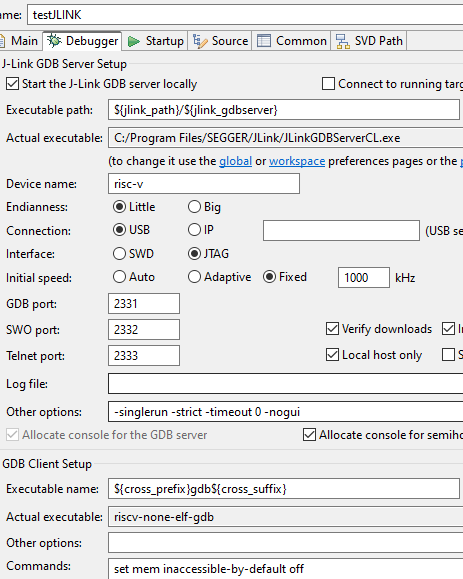
\includegraphics[width=.97\textwidth]{jlink}
		\captionof{figure}{Конфигурација за \textit{J-Link} софтвер}
		\label{fig:jlink}
	\end{minipage}
\end{figure}

Како би програм написан за имплементирани систем могао и да се извршава на њему, неопходно је да постоји неколико помоћних фајлова који се користе при превођењу кода. То су: скрипта за алат \textit{Make}, скрипта за повезивач (енг. \textit{Linker}) и иницијализациони фајл написан у асемблеру. Ови фајлови су базирани на истим који су коришћени при изради \cite{arilla}. Задатак скрипте за \textit{Make} алат је превођење свих фајлова са изворним кодом и потом њихово повезивање коришћењем скрипте за повезивач. Скрипта такође генерише и \textit{.mif} фајл који се може користити за иницијализацију садржаја меморије при конфигурисању \textit{\acrshort{fpga}} чипа, чија је примена примарно у тестирању језгра. При позивању преводиоца, битно је проследити следеће аргументе: \lstinline[language=none,columns=fixed]{-march=rv32i_zicsr -mabi=ilp32 -mstrict-align -nostdlib -ffreestanding} који дефинишиу архитектуру и подршане екстензије, конвенцију позивања, као и да се програм извршава у окружењу без стандардне библиотеке и оперативног система. 
 Скрипта за повезивач дефинише базну адресу и величину меморије, поставља табелу прекидних рутина на право место и дефинише вредности показивача на врх стека, глобалног показивача, почетка и краја секције за неиницијализоване податке. Те вредности се потом користе у иницијализационом фајлу, који дефинише вредности табеле прекидних рутина, дефинише подразумевану и ресет прекидну рутину.
Ресет прекидна рутина уписује вредности глобалног и стек показивача у одговарајуће регистре, иницијализује секцију са неиницијализованим подацима нулама и скаче на \textbf{main} функцију.
Иницијализација секције са неиницијализованим подацима се врши јер при ресетовању језгра садржај меморије остаје исти. Ова поновна иницијализација би требала да се врши и за податке са иницијалним вредностима, међутим то би захтевало постојање две копије тих података у меморији, те та функционалност није имплементирана.  \newpage
\lstinputlisting[language=none,caption=Иницијализациони фајл]{../test/src/startup.s}